\documentclass[crop,convert,tikz]{standalone}
\usetikzlibrary{datavisualization}
\begin{document}
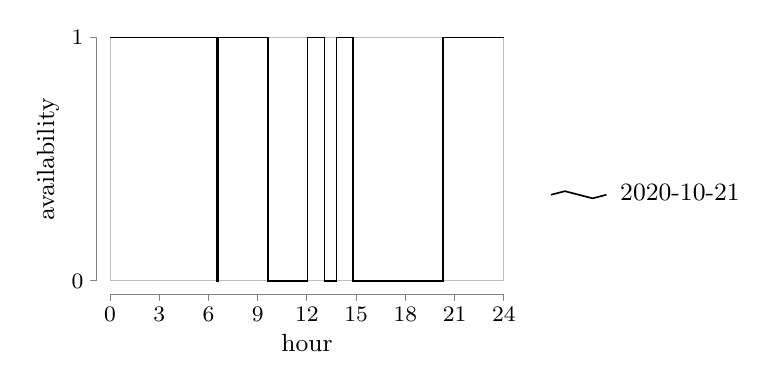
\begin{tikzpicture}
  \datavisualization[
    visualize as line/.list={a,b},
    legend={up then right},
    style sheet=vary dashing,
    scientific axes=clean,
    a={label in legend={text=2020-10-21}},
    x axis={
      label={hour},
      ticks={step=3},
    },
    y axis={
      ticks={major={at={0,1}}},
      label={availability},
    },
  ]
  data [set=a] {
    x, y
    0, 1
    6.48, 1
    6.48, 0
    6.58, 0
    6.58, 1
    9.62, 1
    9.62, 0
    12.04, 0
    12.04, 1
    13.06, 1
    13.06, 0
    13.80, 0
    13.80, 1
    14.82, 1
    14.82, 0
    20.29, 0
    20.29, 1
    24, 1
  };
\end{tikzpicture}
\end{document}
